%
% This is Chapter 7 file (chap7.tex)
%
\chapter{Interplay between linear and non-linear processes} \label{chap:chap7}

    \section{Overview} \label{sec:ovrvw7}

        In the last two chapters, \Cref{chap:chap4} and \Cref{chap:chap5}, we discussed two
        different processes which result in heating or temperature enhancements in the space
        plasmas. As we found in \Cref{chap:chap5} two processes occur simultaneously in both space
        and time and are entangled together at different scales. Consequently, there is an implied
        competition between the two processes to determine which one dominates given a set of
        conditions in the space plasmas. In this chapter we look at the two processes simultaneously
        to see the result of this competition as well as the dynamics between the two. We compare
        the time scales of two processes to see which one dominates and report our results in this
        chapter.\footnote{Part of this study was published in \citet{Bandyopadhyay2020b} and
        \citet{Gary2020}.}

    \section{Introduction} \label{sec:intr7}
    
        Solar wind is weakly collisional. The VDFs of solar wind ions exhibit non-Maxwellian
        features which introduce significant free energy in the system (see \Cref{chap:chap2}). The
        presence of additional features like secondary beam population\footnote{A field aligned
        secondary population of species which moves at a higher speed compared to the core
        population along the magnetic field lines.} \citep[and references therein]{Verscharen2019}
        signifies additional departure from the  local thermodynamic equilibrium and thus provide
        one form of free energy. All this often results in significant departure from temperature
        isotropy ($T_{\perp} = T_{\parallel}$), which leads to the development of kinetic
        microinstabilities\index{microinstability} fueled by the free energy in the system. As discussed in
        \Cref{chap:chap2,chap:chap5}, these instabilities then act to make the system more isotropic
        by scattering of particles in phase space.

        Turbulence is another process by which the opposite affect can be achieved, enhancement in
        anisotropy of the plasma, and because of its ubiquitous nature, it is expected to play
        important role in the dynamics of the plasmas. Thus at any point these two processes are
        either feeding off of each other or are competing in the system. Recent studies have shown
        that coherent structures (e.g., current sheets) generated by solar wind turbulence can
        generate extreme anisotropies \citep{Greco2012,Servidio2015,Karimabadi2013} which results in
        development of linear growth rates as predicted by the Vlasov dispersion equation
        \citep{Qudsi2020a}. Other studies \citep{Karimabadi2013,Matthaeus2015} have shown that local
        instabilities may arise occasionally in the presence of shear driven turbulence\index{turbulence}.
        \citet{Bale2009} found enhancements in magnetic fluctuations in regions of solar wind plasma
        that are susceptible to the development of one or more microinstabilities. \citet{Osman2013}
        showed the presence of high cascade rate in the same regions, suggesting that these two,
        linear and non-linear, processes exist in the same space.

        However, since these two processes compete with each another to influence the plasma, it
        remain unclear as of now which one dominates and drive the large scale phenomenon. We thus
        decided to study the time scales at which the two processes work and compare them in
        different types of plasmas. For kinetic microinstabilities we study the linear growth rates
        (see \Cref{sec:instab2}) whereas for time scales associated with turbulence we look at the
        non-linear frequency and time scales as computed in \Cref{sec:nlts}. We carry out this
        analysis for six different datasets: 3 from simulation and 3 from in-situ measurement of
        space plasmas (see \Cref{chap:chap4} and \Cref{tab:datachap} for details of data and some
        other relevant quantities).

    \section{Data Selection and Methodology} \label{sec:data7}

        Since we are to compare the two time scales, we look at the linear and non-linear rates
        present in the plasma locally. For the linear growth rates, we consider all the four growth
        rates\footnote{Under the assumption of no secondary beam populations and an isotropic
        electron population.} which might be active at any point and compute the maximum of the 4
        rates, where each growth rate was computed by the method described in
        \Cref{sec:cgr,sec:intr42}. \Cref{eq:lin_max_gamma} puts this succinctly in the form of an
        equation.
        \begin{align}
            \Gamma_{\max} & = \max\left( \gamma_{\rm \max, cyclotron}, \gamma_{\rm \max, mirror}, \gamma_{\rm \max, \parallel firehose}, \gamma_{\rm \max, \nparallel firehose} \right) \label{eq:lin_max_gamma}
        \end{align}
        For the non-linear rate, we computed the local nonlinear frequency\index{Frequency!nonlinear} ($\omega_{\rm nl}$) at
        any position \textbf{r} for a lag length scale of $\ell$ as :
        \begin{align}
            \omega_{\rm nl} \sim \delta b_l/\ell \label{eq:nln_time}
        \end{align}
        Where $\delta b_\ell$ is the change in the longitudinal magnetic field and is given by :
        \begin{align}
            \delta b_{\ell} = \left \lvert\hat{\boldsymbol{\ell}} \mathbf{\cdot} \left[\mathbf{b} (\mathbf{r} + \boldsymbol{\ell}) - \mathbf{b} (\mathbf{r})\right]\right\lvert \label{eq:db2},
        \end{align}
        Where \textbf{b} is the total magnetic field expresses in local Alfv\'en speed units (see
        \Cref{sec:nlts}). As mentioned in \Cref{sec:2pic} for all cases except the 3-D dataset,
        since the goal was to carefully evaluate the nonlinear frequency at the scale of the fastest
        growing mode, the value of $\ell$ is given by $1/k_{\max}$, where $k_{\max}$ is the wave
        number corresponding to $\Gamma_{\max}$ as computed in \Cref{eq:lin_max_gamma}. Since for
        marginally unstable plasma, $k_{\max}$ is typically of the same order as the ion inertial
        length ($d_{\rm i}$) \citep[Figures 6.6 to 6.9]{Maruca2012a}, for the case of 3-D
        simulation, because of some computation limitation, we set $\ell = d_{\rm i}$.

    \section{Results} \label{sec:diss7}

        \Cref{fig:ratio_allsim} shows the comparison between the two time scales (linear and
        non-linear) for three different simulations (see \Cref{chap:chap4} for more detail). The
        first panel of each row shows the maximum value of linear growth rates
        $\left(\Gamma_{max}\right)$ as defined by \Cref{eq:lin_max_gamma}. The second panel shows
        the non-linear growth rates $\left(\omega_{\rm nl}\right)$ computed using
        \Cref{eq:nln_time}. Though $\omega_{\rm nl}$ is largely uniform over the simulation box,
        heightened values of it lie close to the regions with high current density and/or where
        temperature anisotropy has extreme values (see \Crefrange{fig:brjhb}{fig:brjros}). The third
        panel shows the ratio between the two growth rates. This ratio is only computed for regions
        where the condition $\Gamma_{\max} > 10^{-5}\Omega_{\rm cp}$ is satisfied, consequently
        there are very few points of comparison compared to the total number of points inside the
        box (see \Cref{tab:ngamma}). The third panel shows that there are very few points where
        $\Gamma_{\max} > \omega_{\rm nl}$, which implies the dominance of non-linear phenomena over
        the linear one for all three different kinds of simulation conditions. This means that it
        takes longer time for the linear instability to affect the system than the eddy turnover
        time and thus it will be the nonlinear processes and not linear instability which will
        dictate the evolution of the system. Counting the number of data points where both the
        conditions ($\Gamma_{\max} > 0$ and $\Gamma_{\max}/\omega_{\rm nl} > 1$) were satisfied, we
        found that the conditions were true only for 0.019, 0.053 and 0.59 percentages of cases for
        \texttt{149p6}, \texttt{kaw} and \texttt{ros} datasets respectively.
        
        \begin{table}[ht]
            \centering
            \caption[Dataset detail for $\Gamma_{\max}$ and $\omega_{\rm nl}$]{Number of points in
            each datasets, and where we have active linear instability present ($\Gamma_{\max} >
            10^{-5}\,\Omega_{\rm cp}$) and where $\Gamma_{\max}/\omega_{\rm nl} > 1$ with associated
            percentages in parenthesis}
            \begin{tabular}{  m{0.15\linewidth}  m{0.25\linewidth}  m{0.25\linewidth}
            m{0.25\linewidth}}
                \hline
                \\
                \multirow{2}{\linewidth}{Datasets} & \multicolumn{3}{|c|}{Number of } \\
                \cline{2-4}
                & total data points & points where \newline $\Gamma_{\max} > 10^{-5}\,\Omega_{\rm
                cp}$ (\%) & points where \newline $\Gamma_{\max}/\omega_{\rm nl} > 1$ (\%)\\
                \hline
                \\
                \texttt{149p6} & 16,777,216 & 1,144,615 (6.82) & 3,347 (0.019)\\ \\
                \hline
                \\
                \texttt{kaw} & 4,194,304 & 37,560 (0.90) & 2,227 (0.053) \\ \\
                \hline
                \\
                %20160125 & & & \\
                %\hline
                \texttt{ros} & 134,217,728 & 22,001,875 (16.39) & 794,220 (0.59) \\ \\
                \hline
                \\
                %20170127 & & & \\
                %\hline
                \texttt{mms} & 15,857 & 3,887 (24.51) & 174 (1.10)\\ \\
                \hline
                \\
                \texttt{wnd} & 1,316,621 & 187,338 (14.22) & 2,7857 (2.11) \\ \\
                \hline
                \\
                \texttt{psp} & 95,034 & 5,347 (5.62) & 1,483 (1.56) \\ \\
                \hline
            \end{tabular}
            \label{tab:ngamma}
        \end{table}

        \begin{sidewaysfigure}
            \begin{center}
                \includegraphics[width=0.95\textheight]{figures/chap7/all_sim_gamma_omega_ratios_blues.pdf}
                \caption[Comparison plot of $\Gamma_{\max}$, $\omega_{\rm nl}$ and
                $\Gamma_{\max}/\omega_{\rm nl}$ for simulations]{Plots (from left to right) of
                maximum linear growth rate ($\Gamma_{\max}$), nonlinear frequency ($\omega_{\rm
                nl}$) and the ratio $\Gamma_{\max}/\omega_{\rm nl}$ for the three different kinds of
                PIC simulation. First row shows the data for \texttt{149p6} dataset, middle row is
                for \texttt{kaw} dataset and the bottom row shows the data from \texttt{ros}
                dataset.}
                \label{fig:ratio_allsim}
            \end{center}
        \end{sidewaysfigure}

        \Crefrange{fig:ratio_mms}{fig:ratio_psp} show the time series equivalent of
        \Cref{fig:ratio_allsim} for three different spacecraft (MMS, Wind and PSP respectively),
        located in different space plasmas: Earth's magnetosheath, 1\,au solar wind, and near-Sun
        solar wind ($\sim$ 0.2\,au) (see \Cref{sec:plas2} and \Cref{chap:chap4}). Similar to
        \Cref{fig:ratio_allsim}, for each of these figure the first panel shows the time series for
        $\Gamma_{\max}$, the second shows that for $\omega_{\rm nl}$, and the third shows ratio of
        the two. The dashed red line in each third panel demarcates $\Gamma_{\max} = \omega_{\rm
        nl}$. Though in all three sets of observations, fraction of data with $\Gamma_{\max} >
        \omega_{\rm nl}$ is higher than in the simulations (see \Cref{tab:ngamma}), it remains well
        below 50\%. Though \citet{Klein2018} used a different method to compute the condition of
        plasma instability and a different condition for calculation of $\omega_{\rm nl}$, they
        found a similar result for solar wind at 1\,au.
        \begin{sidewaysfigure}
            \begin{center}
                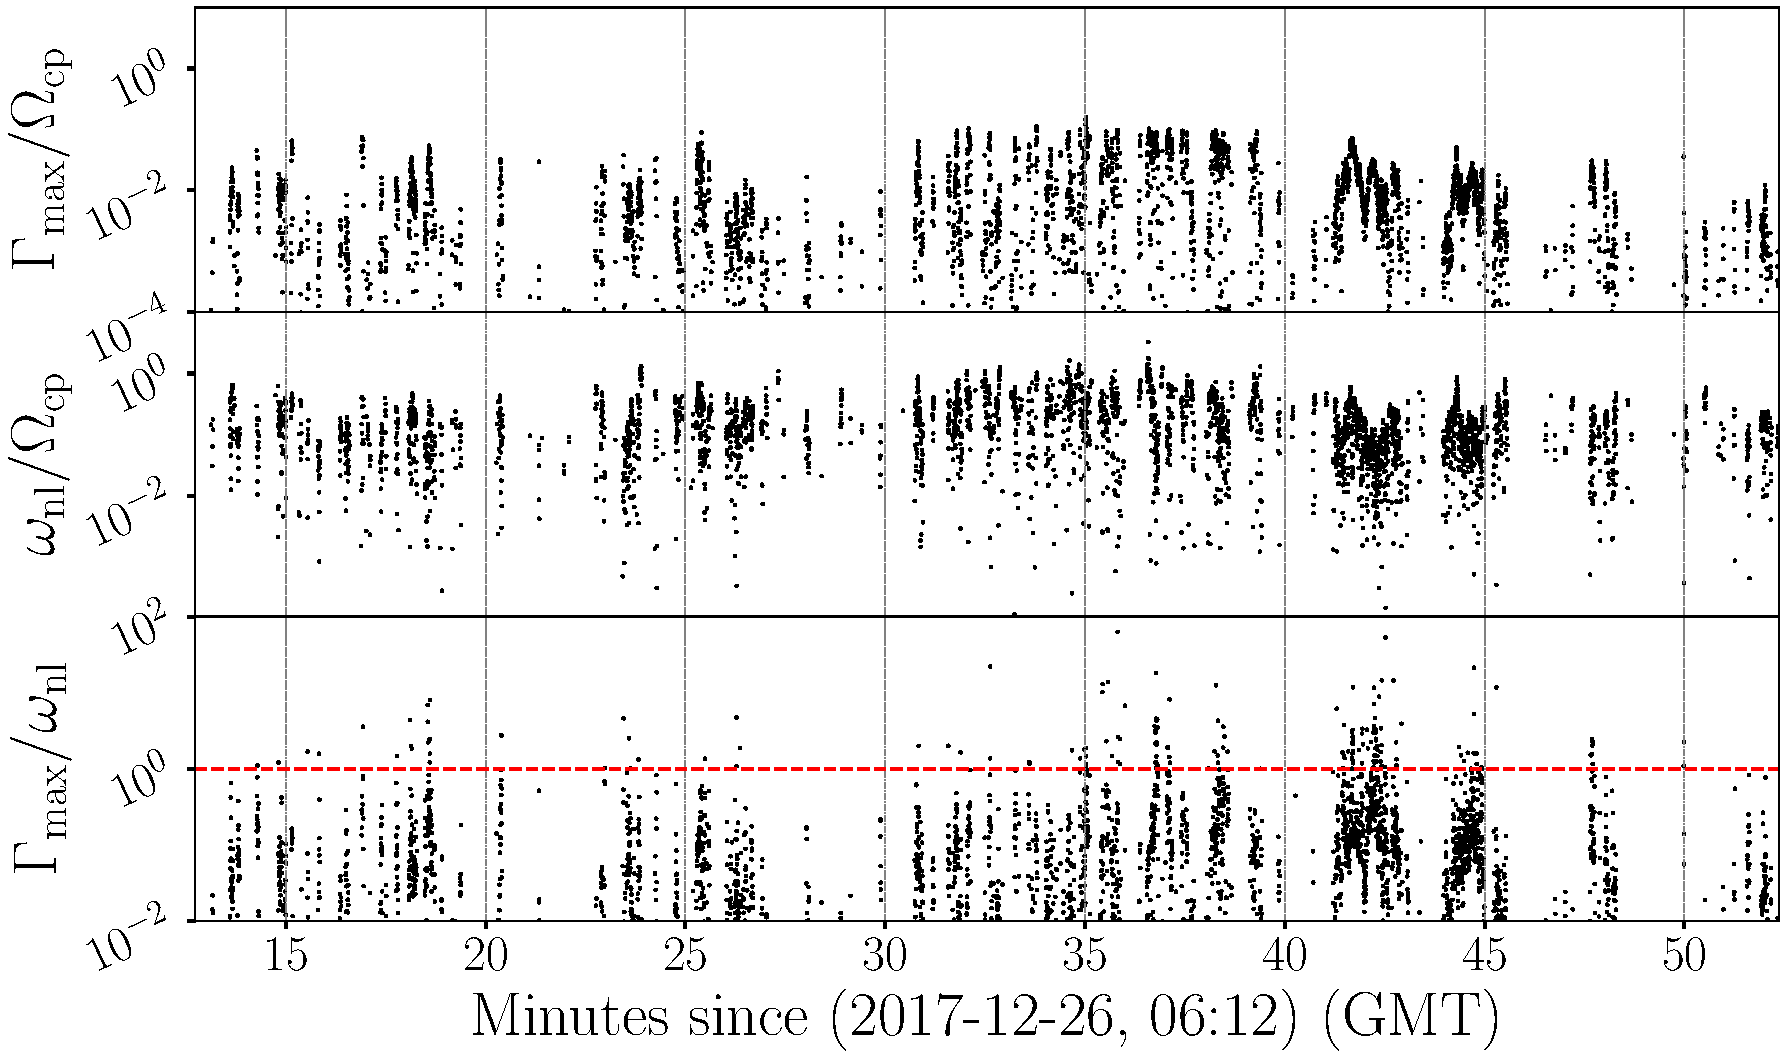
\includegraphics[width=1.\textwidth]{figures/chap7/mms_gamma_omega_ratio_2017-12-26_2017-12-26_00000000_00015856.pdf}
                \caption[Comparison plot of $\Gamma_{\max}$, $\omega_{\rm nl}$ and
                $\Gamma_{\max}/\omega_{\rm nl}$ for \texttt{mms} dataset]{Time series plot of (top
                to bottom) of maximum linear growth rate ($\Gamma_{\max}$), nonlinear frequency
                ($\omega_{\rm nl}$) at 1\,$d_{\rm i}$, and the ratio $\Gamma_{\max}/\omega_{\rm nl}$
                at z\,=\,0.\,$d_{\rm i}$ from terrestrial magnetosheath.}
                \label{fig:ratio_mms}
            \end{center}
        \end{sidewaysfigure}

        \begin{sidewaysfigure}
            \begin{center}
                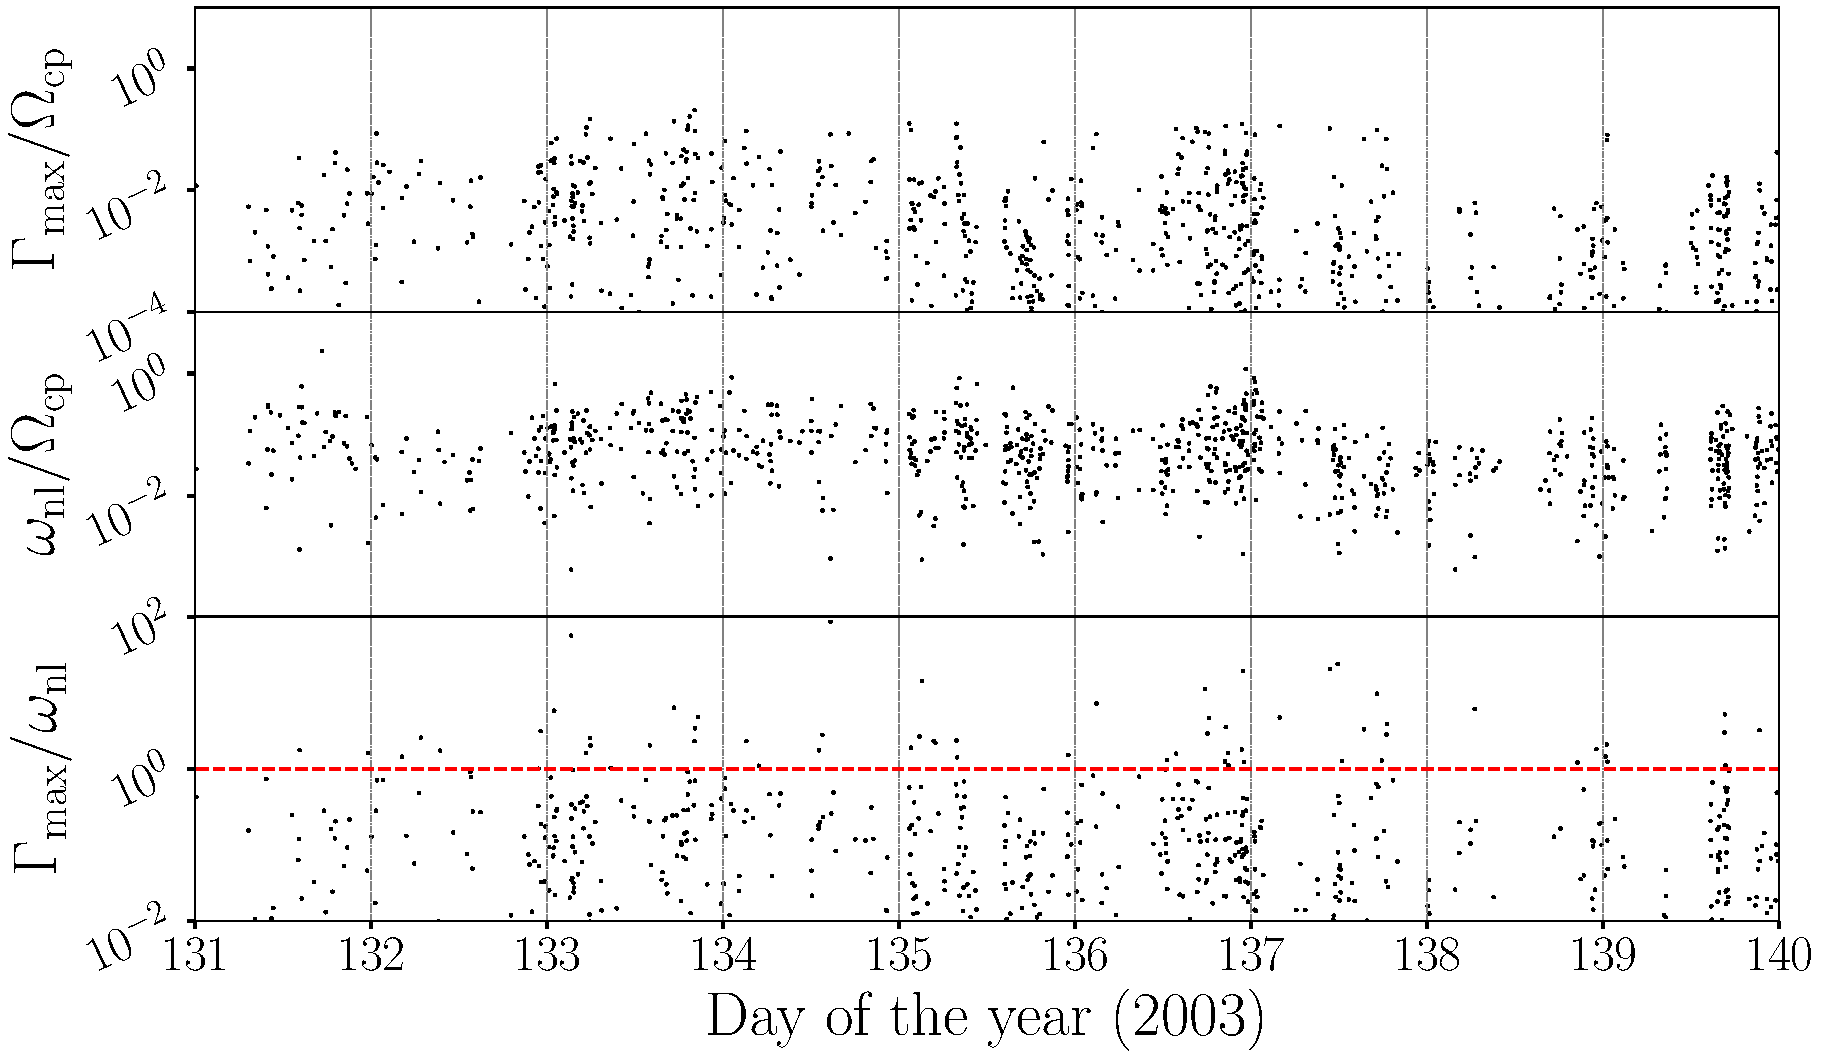
\includegraphics[width=1.\textwidth]{figures/chap7/wnd_gamma_omega_ratio_2003-5-11_2003-5-19_01207878_01212368.pdf}
                \caption[Comparison plot of $\Gamma_{\max}$, $\omega_{\rm nl}$ and
                $\Gamma_{\max}/\omega_{\rm nl}$ for \texttt{wnd} dataset]{Time series plot of (top
                to bottom) of maximum linear growth rate ($\Gamma_{\max}$), nonlinear frequency
                ($\omega_{\rm nl}$) at 1\,$d_{\rm i}$, and the ratio $\Gamma_{\max}/\omega_{\rm nl}$
                at z\,=\,0.\,$d_{\rm i}$ from solar wind at 1-au.}
                \label{fig:ratio_wnd}
            \end{center}
        \end{sidewaysfigure}

        \begin{sidewaysfigure}
            \begin{center}
                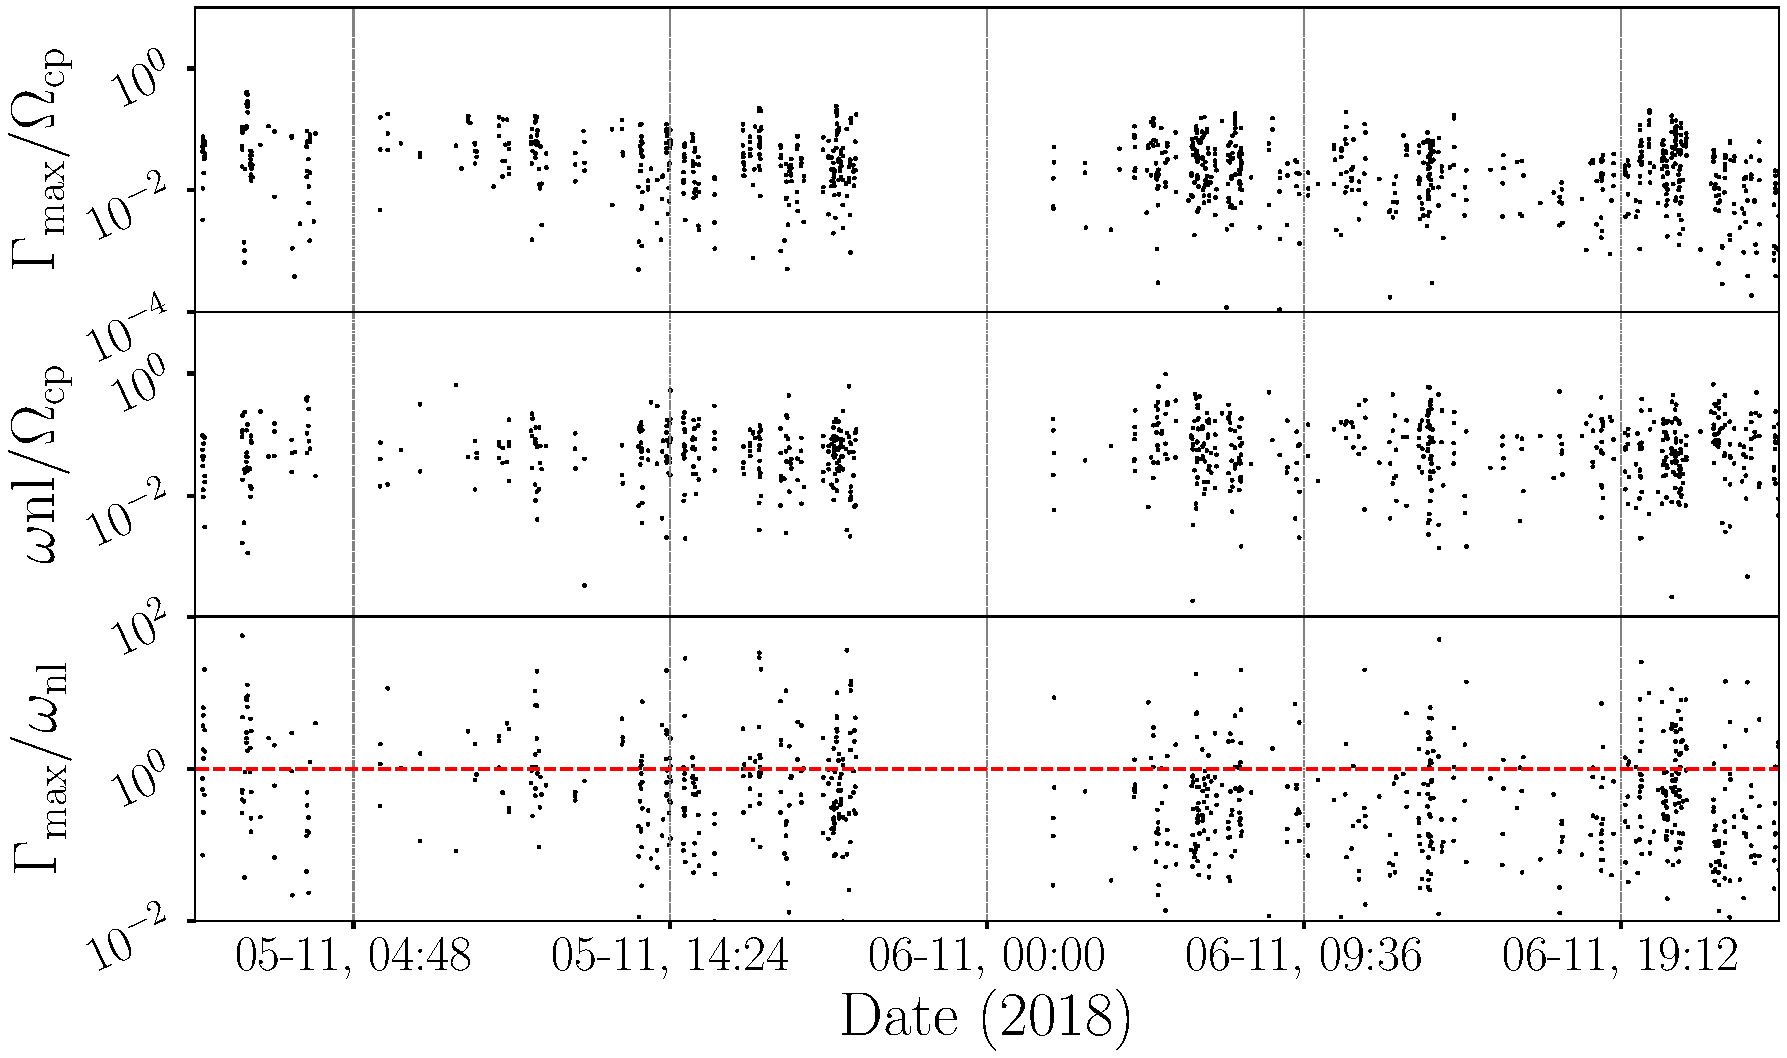
\includegraphics[width=1.\textwidth]{figures/chap7/psp_gamma_omega_ratio_2018-11-5_2018-11-7_00043197_00060477.pdf}
                \caption[Comparison plot of $\Gamma_{\max}$, $\omega_{\rm nl}$ and
                $\Gamma_{\max}/\omega_{\rm nl}$ for \texttt{psp} dataset]{Time series plot of (top
                to bottom) of maximum linear growth rate ($\Gamma_{\max}$), nonlinear frequency
                ($\omega_{\rm nl}$) at 1\,$d_{\rm i}$, and the ratio $\Gamma_{\max}/\omega_{\rm nl}$
                at z\,=\,0.\,$d_{\rm i}$ from solar wind close to the Sun.}
                \label{fig:ratio_psp}
            \end{center}
        \end{sidewaysfigure}
        \Cref{fig:ratio_kde_all} shows the kernel density estimate (KDE) \footnote{KDE is a
        non-parametric method of probability density estimation of a random variable.} plot for each
        of the aforementioned six datasets generated using \texttt{seaborn} package in Python. As
        expected, in all the cases the core of KDE is below $\Gamma_{\max} = \omega_{\rm nl}$ line
        (dashed red line). Though for simulation dataset \texttt{149p6} the core of the distribution
        is centered between $\Gamma_{\max} = 10^{-4}$ and $\Gamma_{\max} = 10^{-3}$, for both
        \texttt{kaw} and \texttt{ros} datasets centroid of KDE is more than an order of magnitude
        higher at $\Gamma_{\max} = 10^{-2}$. This can be attributed to the fact that in both of
        these simulations the background magnetic field ($\mathbf{B_{\rm 0}}$) in the plane of the
        fluctuations is non-zero, by design for the \texttt{kaw} dataset and for \texttt{ros}
        dataset because there are fluctuations in all 3 directions. This results in the case that
        $\textbf{k}_\parallel \neq 0$ for these two simulations, whereas for \texttt{149p6}
        simulation since there is no spatial variation in the direction parallel to $\mathbf{B_{\rm
        0}}$, wave vector components parallel to $\mathbf{B_{\rm 0}}$ are zero. This results in
        limited application of both Landau (fluctuations of zero frequency) and cyclotron resonance
        (fluctuations with $n^{th}$ species cyclotron frequencies)\citep{Gary2020}. This makes both
        the resonances independent of particle velocities and thus the particles are constrained to
        fluid-like behavior. Because of this, \texttt{149p6} simulation fails to account for
        velocity dependent wave-particle interactions which may represent critical elements of
        turbulent dissipation at wavelengths of the order of or shorter than $d_{\rm
        i}$\citep{Gary2020}.
        \begin{sidewaysfigure}
                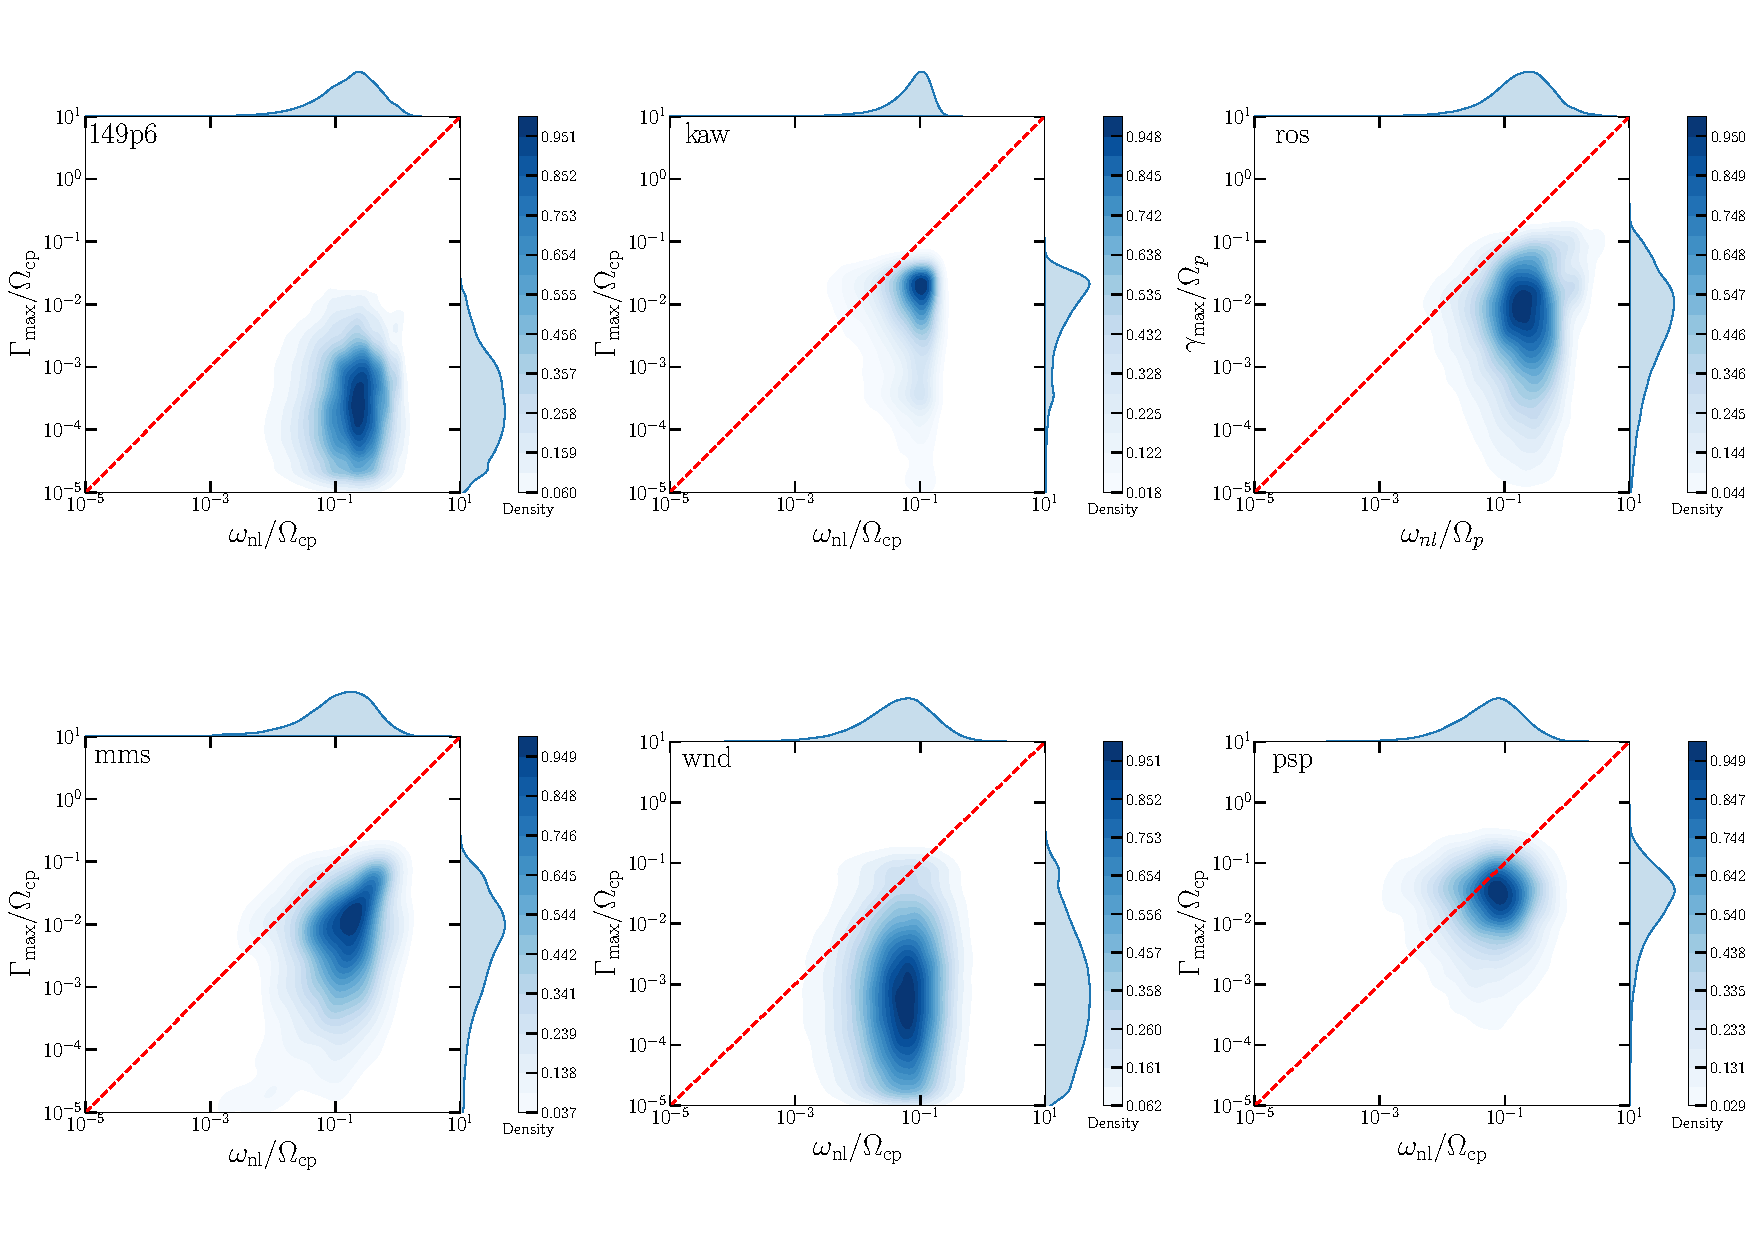
\includegraphics[width=1.\textwidth]{figures/chap7/kdeplots_merged_v9.pdf}
                \caption[KDE plots for all six datasets]{Kernel density plot for all six datasets
                used in this study. For all the cases the centroid of distribution is well below the
                $\Gamma_{\max} = \omega_{\rm nl}$} line, shown as dashed-red line, implying the
                dominance of non-linear processes over linear ones in all kind of plasmas.
                \label{fig:ratio_kde_all}
        \end{sidewaysfigure}
        Another interesting feature of these KDE plots is how much closer to the $\Gamma_{\max} =
        \omega_{\rm nl}$ line the centroid of the distribution is for the PSP data compared to other
        spacecraft data, implying substantially more competition between the linear and non-linear
        processes closer to the Sun. \citet{Klein2021} observed similar enhancements in the linear
        growth rates for plasma closer to the Sun. Further analysis is needed, though, since the
        available PSP data were from such a short time interval (see \Cref{sec:psp}), and
        temperature anisotropy was computed using an entirely novel technique  \citep{Huang2020}. As
        was remarked in \Cref{sec:conc6} close to the Sun the turbulence is quite young and not
        developed enough implying presence of weaker non-linear instabilities. Presence of faster
        linear growth rates closer to the Sun would also explain the stronger-than-expected plasma
        heating as evident in \Cref{fig:tem_pvi_lag}. Another factor could also be the proximity of
        plasma to the Alfv\'en critical region and thus it exhibits wave like bahaviour which are a
        lot stronger than those at 1\,au or in the terrestrial magnetosheath.

        Each of the datasets shows that non-linear time scales are in general faster than linear
        timescales. This would imply that in most cases linear processes never have enough time to
        act on the plasma in a way that is significant enough to affect the dynamics or the
        statistical behaviour of whole plasma. However, as discussed in \Cref{sec:app2} as well as
        in \Cref{sec:conc5}, linear theory is very efficient at predicting the boundaries of
        $(R_{\rm p}, \beta_{\parallel \rm p})$ plots which implies that linear growth rates work
        well enough to regulate extreme values of $R_{\rm p}$ at high $\beta_{\parallel \rm p}$. We
        thus look at the distribution of the two frequencies ($\Gamma_{\max}$ and $\omega_{\rm nl}$)
        and their ratio for the three spacecraft datasets (\texttt{mms}, \texttt{wnd} and
        \texttt{psp}) on the ($R_{\rm p}, \beta_{\parallel \rm p}$) plane.

        \Crefrange{fig:ratio_brz_mms}{fig:ratio_brz_psp} show the distribution of data on a $(R_{\rm
        p}, \beta_{\parallel \rm p})$-plot. The first panel of each figure show the number of data
        points in each bin, the second panel shows the average value of $\Gamma_{\max}$ in each bin,
        $\omega_{\rm nl}$ is shown in the third panel and their ratio in the fourth panel. As
        expected the region along the edges which is most susceptible to instability is where most
        of the instability is present. What is interesting to note is the distribution of
        $\Gamma_{\max}/\omega_{\rm nl}$ along the edges. For all the three spacecraft data, ratio of
        the two frequencies is increasing as we move outside from the centroid (as seen in the first
        panel) distribution. This is evident in all three cases, specially for the solar wind at
        1\,au (\Cref{fig:ratio_brz_wnd}) and near the Sun (\Cref{fig:ratio_brz_psp}) it appears that
        linear time scales are a lot faster than their non-linear counterpart. Signifying that
        though in most cases $\Gamma_{\max} < \omega_{\rm nl}$, it is greater than $\omega_{\rm nl}$
        where it needs to be (along the periphery of $(R_{\rm p}, \beta_{\parallel \rm p})$-plots),
        and thus is quite efficient at limiting the exertion of plasma population to high anisotropy
        regions at high $\beta_{\parallel \rm p}$.

            \begin{sidewaysfigure}
                \begin{center}
                    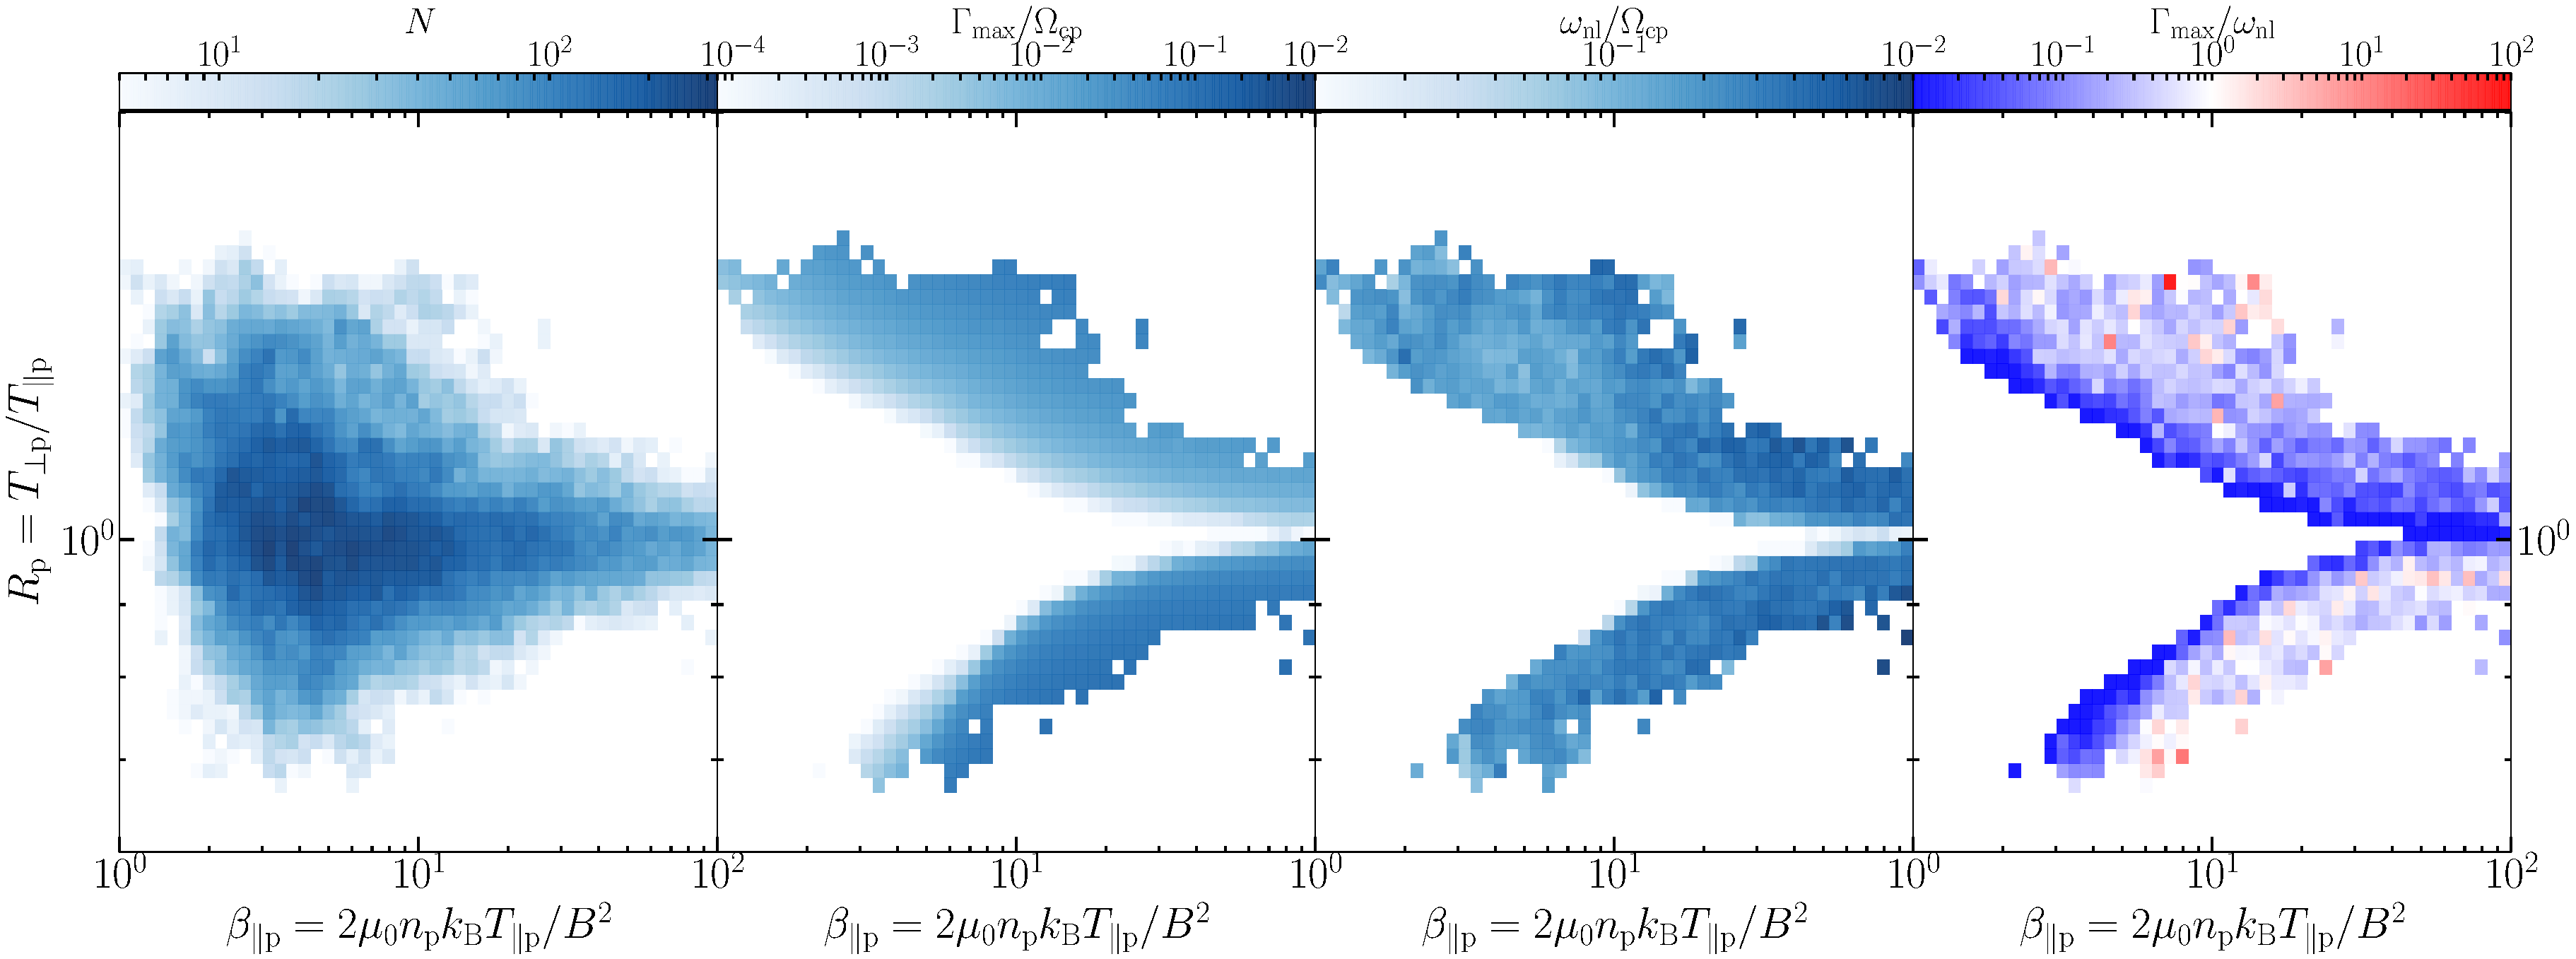
\includegraphics[width=1.\textwidth]{figures/chap7/mms_brz_omega_gamma_mean.pdf}
                    \caption[$(R_{\rm p}, \beta_{\parallel \rm p})$-plot of $\Gamma_{\max}$,
                    $\omega_{\rm nl}$ and $\Gamma_{\max}/\omega_{\rm nl}$ for \texttt{mms}
                    dataset]{$(R_{\rm p}, \beta_{\parallel \rm p})$ plots (from left to right) of
                    distribution of data, maximum linear growth rate ($\Gamma_{\max}$), nonlinear
                    frequency ($\omega_{\rm nl}$), and their ratio ($\Gamma_{\max}/\omega_{\rm nl}$)
                    for earth's magnetosheath.}
                    \label{fig:ratio_brz_mms}
                \end{center}
            \end{sidewaysfigure}

        \begin{sidewaysfigure}
            \begin{center}
                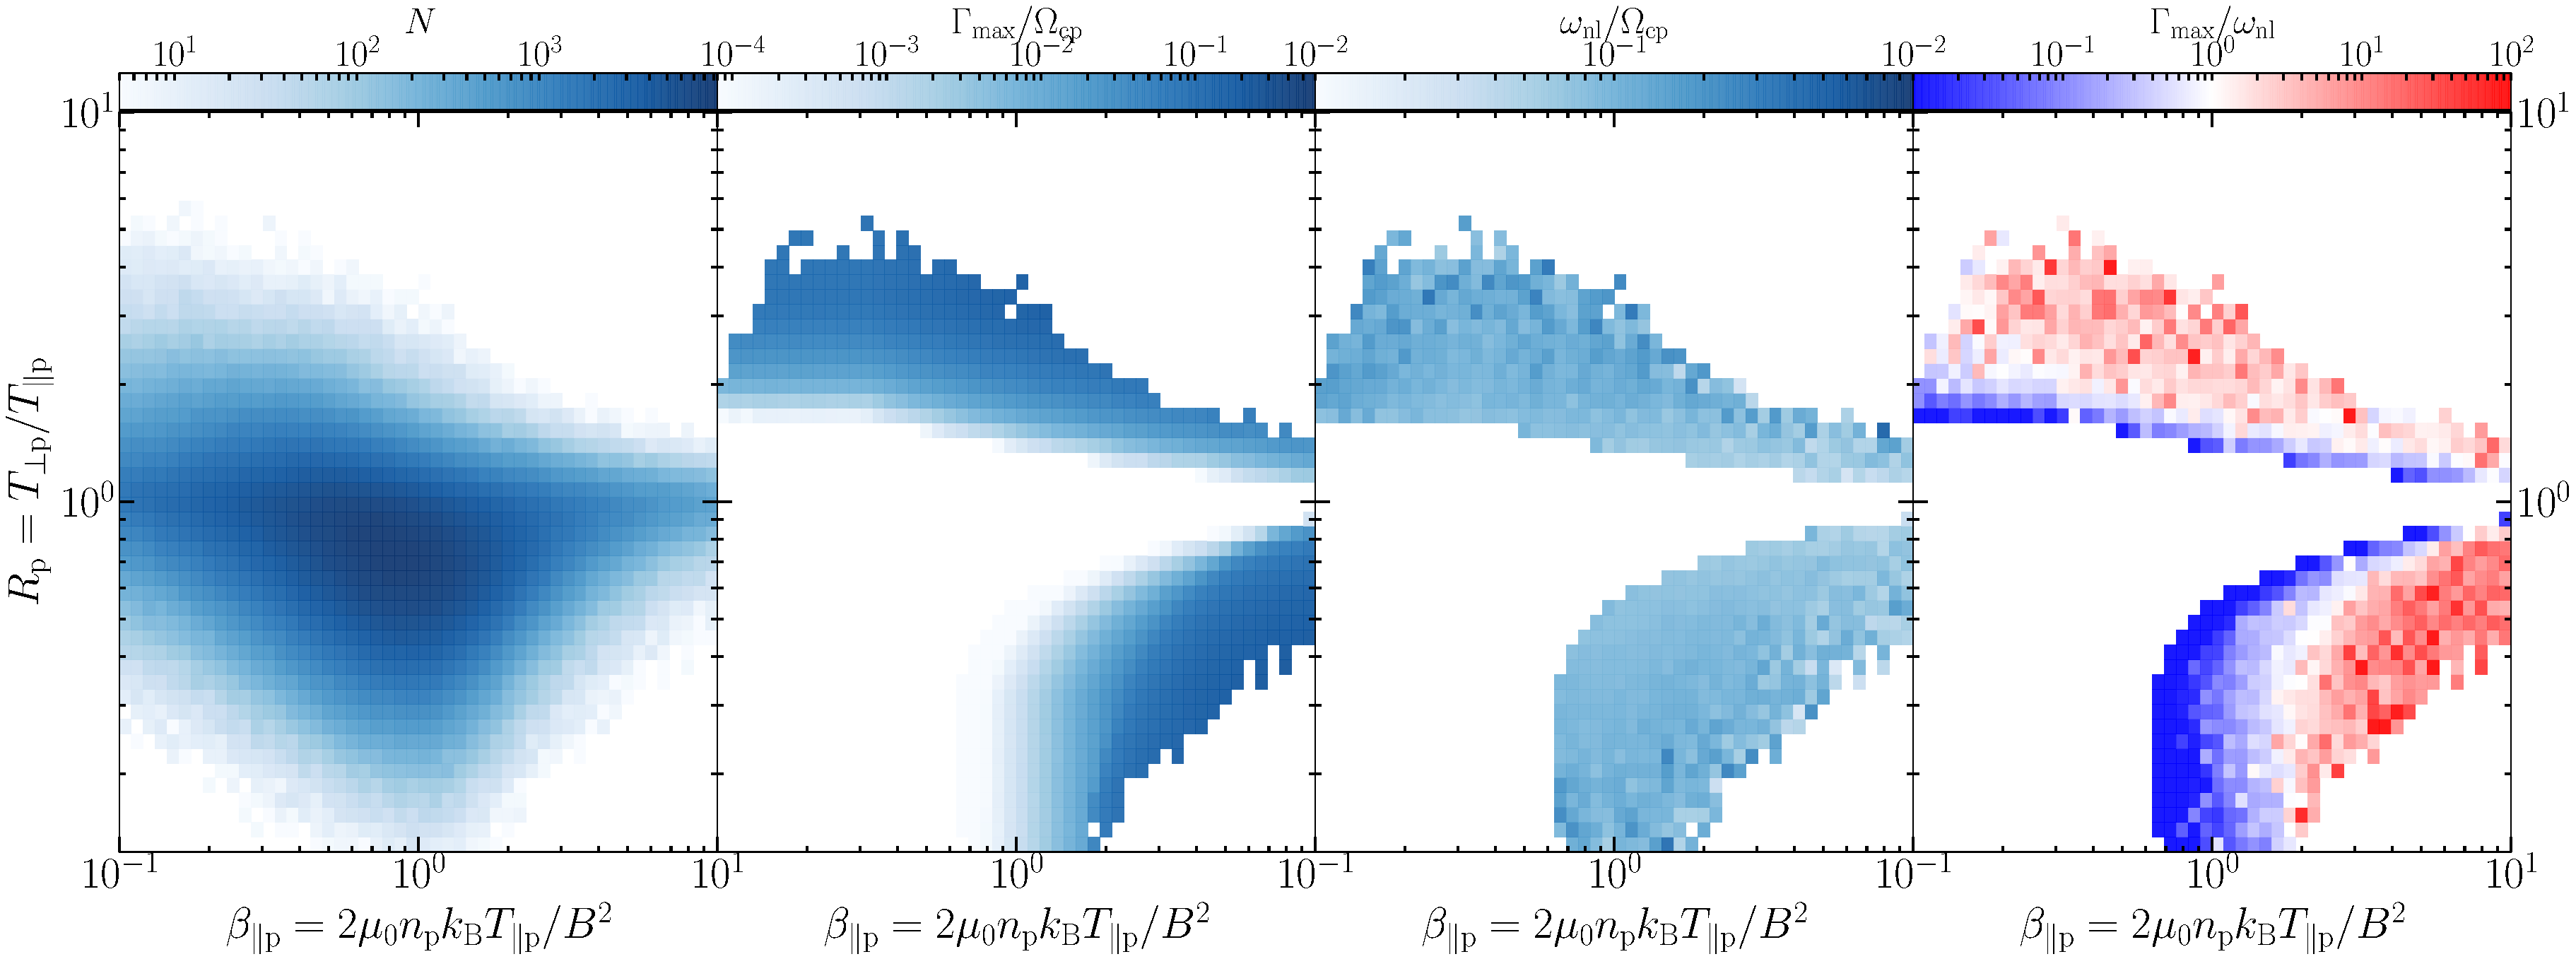
\includegraphics[width=1.\textwidth]{figures/chap7/wnd_brz_omega_gamma_mean.pdf}
                \caption[$(R_{\rm p}, \beta_{\parallel \rm p})$-plot of $\Gamma_{\max}$,
                $\omega_{\rm nl}$ and $\Gamma_{\max}/\omega_{\rm nl}$ for \texttt{wnd}
                dataset]{$(R_{\rm p}, \beta_{\parallel \rm p})$ plots (from left to right) of
                distribution of data, maximum linear growth rate ($\Gamma_{\max}$), nonlinear
                frequency ($\omega_{\rm nl}$), and their ratio ($\Gamma_{\max}/\omega_{\rm nl}$) for
                solar wind at 1-au.}
                \label{fig:ratio_brz_wnd}
            \end{center}
        \end{sidewaysfigure}

        \begin{sidewaysfigure}
            \begin{center}
                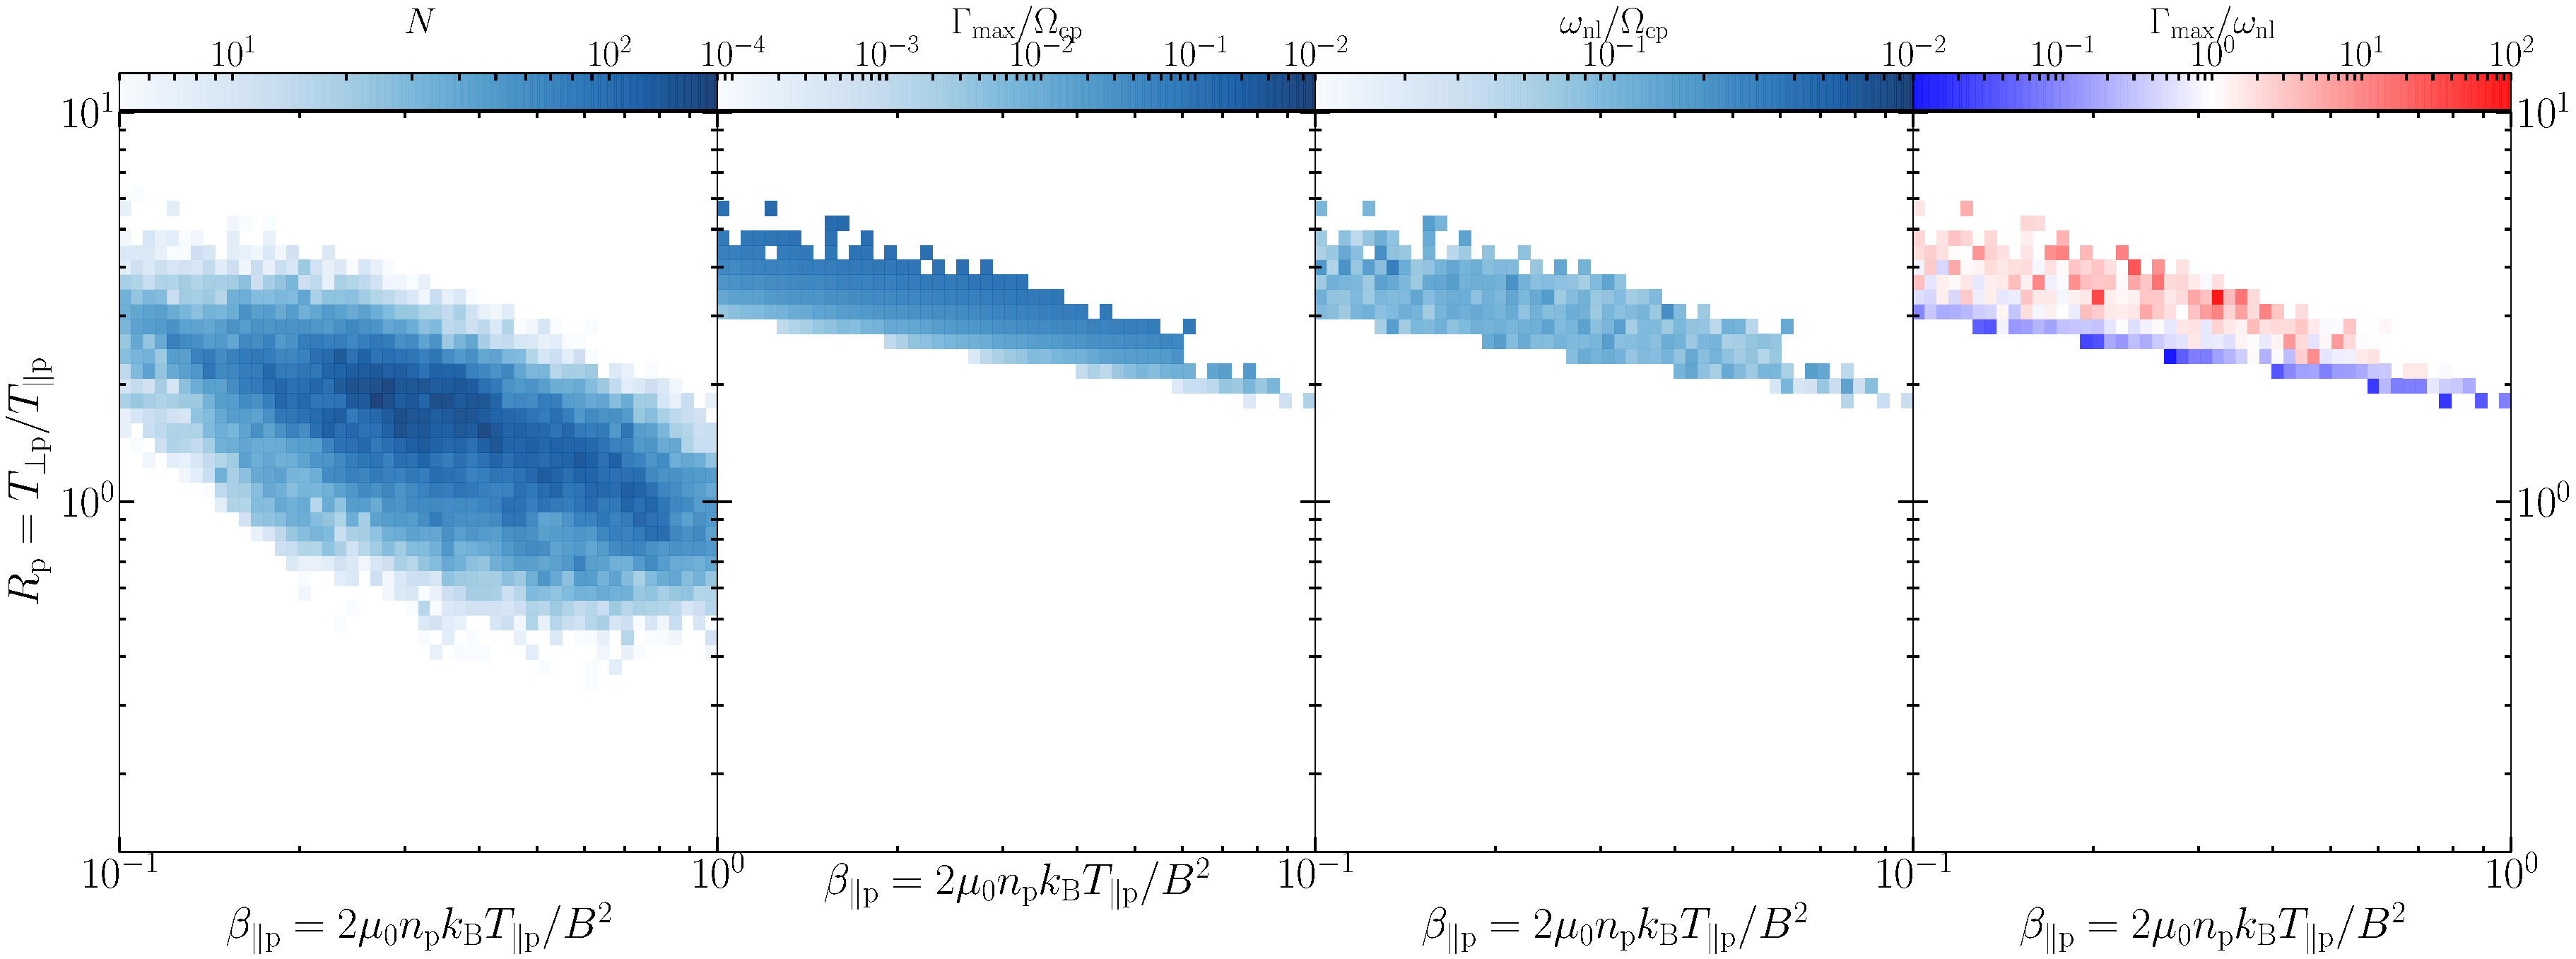
\includegraphics[width=1.\textwidth]{figures/chap7/psp_brz_omega_gamma_mean.pdf}
                \caption[$(R_{\rm p}, \beta_{\parallel \rm p})$-plot of $\Gamma_{\max}$,
                $\omega_{\rm nl}$ and $\Gamma_{\max}/\omega_{\rm nl}$ for \texttt{psp}
                dataset]{$(R_{\rm p}, \beta_{\parallel \rm p})$ plots (from left to right) of
                distribution of data, maximum linear growth rate ($\Gamma_{\max}$), nonlinear
                frequency ($\omega_{\rm nl}$), and their ratio ($\Gamma_{\max}/\omega_{\rm nl}$) for
                solar wind close to the Sun.}
                \label{fig:ratio_brz_psp}
            \end{center}
        \end{sidewaysfigure}

    \section{Discussions} \label{sec:conc7}

        We investigated the competition between linear and non-linear time scales for 6 different
        datasets. We observed that non-linear processes arising because of turbulence dominate
        linear ones overwhelmingly (\Crefrange{fig:ratio_allsim}{fig:ratio_psp}). This would imply
        that the linear processes are of little consequence as far as dynamics and statistical
        properties of a turbulent plasmas is concerned. Yet, in-situ observations of space plasmas
        present strong evidence that linear microinstabilities regulate ion temperature anisotropy.
        Multiple studies of in-situ observations
        \citep{Gary1991,Gary1994,Gary2001,Gary2006,Kasper2002,Hellinger2006,Maruca2011,Maruca2012,Maruca2018},
        have found that the distribution of plasma over the ($R_{\rm p}, \beta_{\parallel \rm p}$)
        plane well restricted by thresholds predicted by linear Vlasov theory\index{Vlasov} one must conclude that
        linear theory works. Observations made in \Crefrange{fig:ratio_brz_mms}{fig:ratio_brz_psp}
        provide further evidence. We observed that though $\omega_{\rm nl} > \Gamma_{\max}$ for most
        part, along the lines of threshold where microkinetic instabilities are most active, linear
        processes disrupt the turbulence cascade and dominate. However, as we saw in
        \Cref{fig:ratio_brz_mms} even when the two processes have comparable values along the edges,
        it still gave rise to expected $(R_{\rm p}, \beta_{\parallel \rm p})$ plot
        \citep{Maruca2018}. Recent studies have shown that regions of extreme temperature anisotropy
        are produced because of generation of sharp gradients by turbulence
        \citep{Osman2011,Greco2012,Valentini2014,Parashar2016}, and we know that kinetic
        microinstabilities are most active where $R_{\rm p}$ deviates significantly from unity.
        \citet{Osman2013} showed that turbulence cascade rates are highest along the edges as well.
        All this indicates a complicated interplay between turbulent and microkinetic phenomena.

        In this chapter we compared linear growth rates derived using linear dispersion relation
        under the assumption of homogeneity of background fields. An ideal method would involve
        computation of $\gamma$ based on theory which takes such inhomogeneities as are present in
        plasmas into account. Understanding the kind of turbulence present in the system can further
        assist us in an accurate computation of $\omega_{\rm nl}$. Since it is extremely difficult
        to gauge the kind of turbulence present in a system without the knowledge of magnetic
        structure a full 3-D image of magnetic field can help substantially. Though development of
        linear theory based on inhomogeneities has been deferred to future work, in
        \Cref{chap:chap8} we discuss a probable future mission and proof of concept for measuring
        full 3-D structure of magnetic field from kinetic to mesoscales at 1\,au.